\documentclass[xcolor=dvipsnames]{beamer}
%\usetheme{Pittsburgh}
\usepackage{pgfpages}
\usepackage{graphicx}
\usepackage{colortbl}
\usepackage{tikz}
\usepackage{pgfplots}
\usepackage{booktabs}
\usepackage[abs]{overpic}
\usepackage[scientific-notation=true]{siunitx}
\usetikzlibrary{decorations.pathreplacing}
\usetheme{MarburG}
\usecolortheme{whale}
\usepackage[ngerman]{babel}
\usepackage[utf8]{inputenc}
\newcommand{\pro}{\item[\boldmath${\color{green}+}$ ]}
\newcommand{\con}{\item[\boldmath$ {\color{red}-}$ ]}
\usetikzlibrary{shapes.misc}
\usetikzlibrary{calc}
\tikzset{cross/.style={cross out, draw=red, minimum size=2*(#1-\pgflinewidth), inner sep=0pt, outer sep=0pt},
%default radius will be 1pt. 
cross/.default={1mm}}

\let\oldfootnotesize\footnotesize
\renewcommand*{\footnotesize}{\oldfootnotesize\tiny}

\newcommand{\tikzmark}[1]{\tikz[overlay,remember picture] \node (#1) {};}
\newcommand{\DrawBox}[1][]{%
    \tikz[overlay,remember picture]{
    \draw[red,#1]
      ($(left)+(-0.84cm,0.9cm)$) rectangle
      ($(right)+(-0.22cm,-0.2cm)$);}
}

%\setbeameroption{hide notes} % Only slide
%\setbeameroption{show only notes} % Only notes
%\setbeameroption{show notes}
\setbeameroption{show notes on second screen=left} % Both

\title{Last-Tests von Webseiten mit JMeter}
\subtitle{Seminararbeit SS 2018}
\titlegraphic {
\includegraphics[width=2cm]{bilder/hskalogo_only}}
\author{Daniel Schäfer}
\date{\today}

%----------------------------------------------------------------------
\begin{document}

%titelseite------------
\begin{frame}
\titlepage
\end{frame}
%----------------------

%inhaltsverzeichnis----
\begin{frame}
\frametitle{Agenda}
		\tableofcontents
\end{frame}
%----------------------

%-------1--------------
\section{Einleitung}
\begin{frame}
\frametitle{Einleitung}
%\begin{overpic}[width=1\textwidth, grid, tics=10]{bilder/elephants}
\begin{center}\begin{overpic}[width=1\textwidth]{bilder/elephants}
\put(10, 80){\tiny Bildquelle: https://www.businessnewsdaily.com/6620-what-work-life-balance.html}
\end{overpic}
\end{center}

\note{bild fand ich ganz passend. es stammt aus einem work life balance artikel aber trifft lasttest ganz gut. worum geht es? ich will kurz die motiviation ansprechen. wozu braucht man lasttests, danach basiswissen von lasttests vermitteln und was für anforderungen man benötigt.}
\end{frame}
%----------------------

%-------1.1------------
\subsection{Motivation}
\begin{frame}
\frametitle{Motivation}
\begin{center}
\includegraphics[angle=10, width=0.7\textwidth]{bilder/unerreichbar}
\end{center}
IWI-Intranet Seite geht am Anmeldetermin der Seminar/Projektarbeiten unter der Last in die Knie! 
\note{Weitere beispiele wie Neue Webseite oder Shop die viele Besucher erwartet, hat große Latenzzeiten oder
ist gar nicht mehr erreichbar (Worst Case)}
\note{Greg Linden - Amazon hat ermittelt, dass sie pro 100ms verzögerung 1\% weniger verkaufserlöse haben. Daraus folgt Zeit = Geld / schneller = besser}
\end{frame}
%----------------------

%-------1.2.1----------
\subsection{Grundlagen Lasttests}
\begin{frame}
\frametitle{Grundlagen Lasttests}
\textbf{Was sind Lasttests?}\newline
Bei einem Lasttest wird hohe Last auf einem System erzeugt und das Verhalten untersucht. Ziel:
\begin{itemize}
		\item Erfüllung nicht funktionaler Anforderungen wie Antwortzeiten / Mengenbewältigung
		\item Dimensionierung von Hardwareresourcen  	
		\item Aufdeckung nicht gefundener Fehler (Nebenläufigkeit und blockierende Prozesse)
\end{itemize}
\textbf{Wozu Lasttests?} \newline Stabilität der Anwendung prüfen
\end{frame}
%----------------------

%-------1.2.2----------

\begin{frame}
\frametitle{Grundlagen Lasttests}

\textbf{Manuelles Testen}
\begin{itemize}
\item "`echte"' Personen bedienen die Anwendung
\item Zeit- und resourcenintensiv \newline
\note{Man benötigt einige Benutzer, in kleineren Firmen oft die Entwickler selbst, die in dem Zeitraum nicht zur Verfügung stehen. man verwechselt häufig Lasttests mit UAT. user akzeptanztests sollten schon gemacht werden. allerdings mehr auf funktionalität bezogen und weniger auf die Last}
\end{itemize}

\textbf{Automatisiertes Testen}
\begin{itemize}
\item Tools wie JMeter
\item Simulation von vielen Benutzern (Threads)
\note{achtung man sollte parametrisierte werte wie passwörter/benutzernamen (base64) oder eventuelle captchas (einheitlich) im vorfeld beachten. } 
\end{itemize}
\end{frame}

%-------1.3------------
\subsection{Anforderungen an Lasttests}
\begin{frame}
\frametitle{Anforderungen an Lasttests}
Lastvarianten (Gleichzeitig, AKtiv, Spitze)
Antwortzeiten und Durchsatz
Infrastruktur Hardware
\end{frame}
%----------------------

%-------2--------------
\section{Apache JMeter}
\begin{frame}
\frametitle{Apache JMeter}
\begin{center}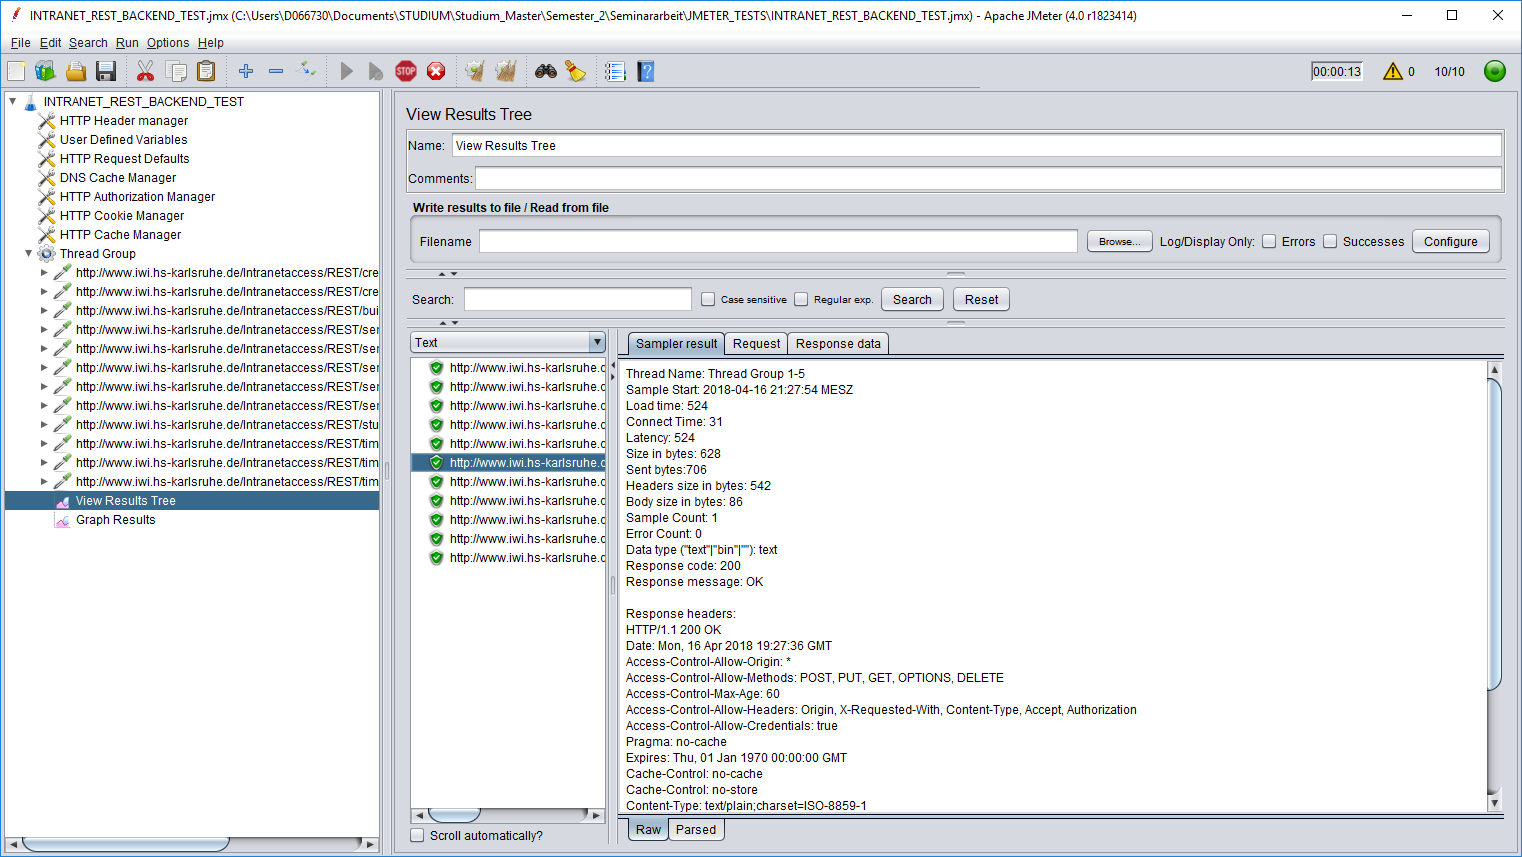
\includegraphics[width=1\textwidth]{bilder/jmeter_1}
\end{center}
\note{JMeter ist ein open source Lasttestprogramm von Apache und wurde von Stefano MAzzocchi entwickelt um die performance von Apache Tomcat zu testen. Hat sich daraufhin stetig weiterentwickelt und ist heute bei großkonzernen wie sap und 1und1 regelmäßig im einsatz und den resourcenbedarf von anwendungen zu ermitteln. auf die hier abgebildete gui wird später genauer eingegangen }
\end{frame}
%----------------------


%-------2.1------------
\subsection{JMeter Übersicht}
\begin{frame}
\frametitle{JMeter Übersicht}

\begin{itemize}
\item Open Source / platformunabhängig (Java-Anwendung)
\item JMeter erzeugt Anfragen und somit Last auf Servern
\item Kann sehr viele Protokolle wie HTTP (SOAP/REST), JDBC, FTP, ..
\item GUI + Non-GUI-Modus
\item Kann Benutzer (Threads) simulieren
\item Master-Slave-fähig für Cloud-Anwendungen
\item Umfangreiche Reporting Funktionen
\end{itemize}
\end{frame}
%----------------------

%------2.2.1-----------
\subsection{Funktionsweise von JMeter}
\begin{frame}
\frametitle{Funktionsweise von JMeter}
\begin{itemize}
\item Erstellung eines Skripts durch Aufzeichnen von Browserinteraktionen
\item Parametrisierung z.b. durch Anzahl Benutzer, Benutzernamen, Passwörter, Servernamen, Ports
\item Test ausführen und anschließend analysieren 
\note{Analyse dann durch Reports}
\end{itemize}
\end{frame}
%----------------------

%------2.2-------------
\subsection{Die JMeter GUI}
\begin{frame}
\frametitle{Die JMeter GUI}
\end{frame}
%----------------------

%------2.3-------------
\subsection{JMeter Elemente}
\begin{frame}
\frametitle{JMeter Elemente}
\end{frame}
%----------------------

%-------2--------------
\section{Live Demo}
\begin{frame}
\frametitle{Live Demo}
\begin{itemize}
	\item Test von 10k Threads im GUI Modus mit Graph 
	\item HTML Dashboard mit Konsolenaufruf
\end{itemize}
\end{frame}
%----------------------

 
\section{Fazit}
\begin{frame}
\frametitle{Fazit}
\end{frame}

\subsection{Vor- und Nachteile}	
\begin{frame}
	\frametitle{Vor- und Nachteile}
	\begin{itemize}
		\pro Platformunabhängig
		\pro Testerstellung in GUI
		\pro Testlauf in GUI/Kommandozeile
		\pro Ergebnisse in HTML Dashboard
		\pro Timer um Tests zu automatisieren
		
		\con Swing Oberfläche
		\con Testpläne in XML-Format \note{JMX Format ist eine XML Datei. Daher unhandlich ohne GUI werte zu ändern}
		\con GUI resourcenhungrig
	\end{itemize}
\end{frame}

\subsection{Abschließende Worte}
%\subsection{Ausblick}
\begin{frame}
\frametitle{Abschließende Worte}

\note[item]{Lasttests sind nach wie vor ein zweischneidiges schwert. in den zeiten von TDD ist der fokus vermehrt wieder testen gerückt. allerdings nur in richtung unit/component/integration testing. lasttests fristen nach wie vor ein nischendaschein und JMeter und konsorten werden leider viel zu selten in der entwicklung eingesetzt. denn nach wie vor ist es immer noch wichtiger, dass ein produkt erst fertig wird (aufgrund von zeitdruck und knappem budget) als resourcen in optimierung zu setzen}

	Die Funktionalität einer Anwendungen steht immer an erster Stelle. Erst wenn alle Anforderungen des Kunden erfüllt sind und noch Zeit/Budget vorhanden ist wird optimiert! 
	\end{frame}


\end{document}



FRAGEN:
live test des programms? recording nicht, aber z.b. test der iwi seite mit 10000 benutzern und live graph? danach noch das dashboard.
alternativprogramme erwähnen, auch wenn man die nicht getestet hat. oder noch testen/ganz weglassen?